\documentclass[12pt,letterpaper]{article}
\usepackage{graphicx,textcomp}
\usepackage{natbib}
\usepackage{setspace}
\usepackage{fullpage}
\usepackage{color}
\usepackage[reqno]{amsmath}
\usepackage{amsthm}
\usepackage{fancyvrb}
\usepackage{amssymb,enumerate}
\usepackage[all]{xy}
\usepackage{endnotes}
\usepackage{lscape}
\newtheorem{com}{Comment}
\usepackage{float}
\usepackage{hyperref}
\newtheorem{lem} {Lemma}
\newtheorem{prop}{Proposition}
\newtheorem{thm}{Theorem}
\newtheorem{defn}{Definition}
\newtheorem{cor}{Corollary}
\newtheorem{obs}{Observation}
\usepackage[compact]{titlesec}
\usepackage{dcolumn}
\usepackage{tikz}
\usetikzlibrary{arrows}
\usepackage{multirow}
\usepackage{xcolor}
\newcolumntype{.}{D{.}{.}{-1}}
\newcolumntype{d}[1]{D{.}{.}{#1}}
\definecolor{light-gray}{gray}{0.65}
\usepackage{url}
\usepackage{listings}
\usepackage{color}
\usepackage{longtable}
\usepackage{pdflscape} 
\usepackage{rotating}
\usepackage{tabularray}
\usepackage{siunitx}
\UseTblrLibrary{siunitx}
\UseTblrLibrary{booktabs}

\definecolor{codegreen}{rgb}{0,0.6,0}
\definecolor{codegray}{rgb}{0.5,0.5,0.5}
\definecolor{codepurple}{rgb}{0.58,0,0.82}
\definecolor{backcolour}{rgb}{0.95,0.95,0.92}

\lstdefinestyle{mystyle}{
	backgroundcolor=\color{backcolour},   
	commentstyle=\color{codegreen},
	keywordstyle=\color{magenta},
	numberstyle=\tiny\color{codegray},
	stringstyle=\color{codepurple},
	basicstyle=\footnotesize,
	breakatwhitespace=false,         
	breaklines=true,                 
	captionpos=b,                    
	keepspaces=true,                 
	numbers=left,                    
	numbersep=5pt,                  
	showspaces=false,                
	showstringspaces=false,
	showtabs=false,                  
	tabsize=2
}
\lstset{style=mystyle}
\newcommand{\Sref}[1]{Section~\ref{#1}}
\newtheorem{hyp}{Hypothesis}

\begin{document}
	
	\begin{titlepage}
		\centering
		{\LARGE\bfseries Replication Project}
		
		\vspace{1cm}
		
		{\Large Who Shot the Bullets? Exposure to Violence and Attitudes Toward Peace: Evidence from the 2016 Colombian Referendum}
		
		\vspace{1cm}
		
		{\normalsize Rosalie LaCroix}
		
		{\normalsize Applied Stats II}
		
		{\normalsize Due: April 2, 2026}
	\end{titlepage}
	
	
	\section*{1. Original Study}
	
	The study I have chosen to replicate is "Kreiman, G., \& Masullo, J. (2020). Who Shot the Bullets? Exposure to Violence and Attitudes Toward Peace: Evidence from the 2016 Colombian Referendum. Latin American Politics and Society, 62(4), 24–49. doi:10.1017/lap.2020.14". 
	
	This study explores a potential reasoning behind the surprising results of the 2016 Peace Referendum in Colombia. The referendum was brought to a public vote in 2016 by the Colombian president Juan Manuel Santos, following peace talks and a subsequent ceasefire agreeement between the Colombian government and the Revolutionary Armed Forces of Colombia (referred to as "FARC" from this point forward). FARC were known as the largest and most powerful guerilla group operating throughout the 50 years of the Colombian civil war. The referendum also included provisions for rural reform, strategies to reduce coca growth and drug trafficking, as well as the allowance of FARC participating in elections. The public vote resulted in the referendum not being passed by an incredibly small margin. Santos and FARC subsequently continued negotiations and Santos passed the referendum through Colombian congress in late 2016.
	
	Due to surprising results of the public referendum vote, researchers began to explore why this might have been the case. Preliminary research determined that there were clear geographical patterns within the votes, which was also a case for the patterns of violence throughout the war. Subsequent hypotheses have stated that support for the referendum was higher in areas more strongly impacted by war-time violence, as well as that areas under FARC control voted against the referendum due to the fact that it did not appear punish FARC enough. Ultimately, there has been a great amount conflicting beliefs on why the referendum did not go through on the public vote. Kreiman and Masullo discovered a gap in the research regarding how variation in people's experiences of violence might have impacted their attitudes towards peace. They hypothesized that the identity of the perpetrator matters in how people are affected by violence and their subsequent attitude towards peace. Specifically, that individuals in municipalities more impacted by FARC violence were more supportive of the referendum, whereas people more impacted by paramilitary violence were less supportive. The main paramilitary group considered in this investigation was BACRIM (criminal bands in spanish), a paramilitary group formed following the demobilization of the United Self Defence Forces of Colombia (AUC). The AUC was a paramilitary group formed in the 1980s to combat the advancements of FARC.
	
	\vspace{.5cm}
	
	\textbf{Hypotheses:}
		\begin{itemize}
			\item In areas where Group A has committed most of the violence, residents are more likely to support a peace agreement with Group A.
			\item In areas where B has committed most of the violence, residents are less likely to support a peace agreement with Group A.
		\end{itemize}
	
	\newpage
	\textbf{Method:}
	
	In order to determine how violence perpetrated by FARC and/or paramilitaries/BACRIM impacted the victims' votes in the 2016 referendum, Kreiman and Masullo gathered previously collected data on overall exposure to violence in municipalities through Colombia, number of attacks perpetrated by each group in each municipality, the percentage of votes per municpality supporting the referendum, as well as various control variables. This was a quantitative study utilizing an ordinary least squares regression with departmental fixed effects to make inferences regarding their research question and hypotheses. 
	
	\vspace{.8cm}

	\section*{2. Data}
	
	\lstinputlisting[language=R, firstline=38, lastline=43]{replication_r_code.R}
	
	\textbf{Outcome Variable:}
	\begin{itemize}
		\item \% of votes per municipality supporting the 2016 peace agreement referendum
	\end{itemize}
	
	\textbf{Independent Variables:}
	
	\noindent Set of variables measuring the average number of violent attacks carried out by FARC and paramilitaries/BACRIM from the years 1988-2010.
	\begin{itemize}
		\item (ln) FARC attacks
		\item (ln) Paramilitary/BACRIM attacks
	\end{itemize}
	
	\textbf{Control Variables:}
	
	\noindent Set of variables that could have an impact on perceived violence and voting in referendum, including political influences, socioeconomic and demographic influences, and variability of natural resources.
	\begin{itemize}
		\item \% Votes for Santos in 2014 Election
		\item \% Participation in Referendum
		\item Poverty Measure
		\item Population Measure
		\item Rurality Index
		\item Coca Cultivation
		\item Oil Present
		\item Elevation
		\item Education
	\end{itemize}
	
	\textbf{Fixed Effects:}
	
	A fixed effects model was utilized to control for unobserved characteristics that do not change over time and are specific to each department, as Colombia consists of 32 departments and one capital district (Bogota). For the purpose of departmental fixed effects, Bogota was considered its own department. This model added a dummy variable for each department, allowing each to have its own unique intercept.
	
	\vspace{.8cm}
	
	\section*{3. Original Model}
	
	\noindent The authors utilized Stata, which has a wildcard variable denotation to match naming patterns, which the authors used to capture the 33 department in their formula. As R does not have this capability, I created an object that included all of the departments that I pasted onto each formula.
	
	\lstinputlisting[language=R, firstline=47, lastline=48]{replication_r_code.R}
	
	\noindent There is an incredibly important note that must be made prior to the presentation of the replication code. The authors did not use a consistent reference category for the department dummy variable. Stata typically utilizes the same default reference category as R, which is the lowest-valued category, but upon replicating the regression this did not appear to be the case. For this reason, I created a loop that determined the reference category for each of the 7 models that were run. This loop compared the intercept value obtained using each reference category to the one presented for that model by the authors until it found the reference category that resulted in an intercept within 0.01 from that in the paper.
	
	\vspace{.5cm}
	
	\noindent\textbf{Model 1: FARC Attacks Only}
	
	\lstinputlisting[language=R, firstline=51, lastline=68]{replication_r_code.R}
	
	\noindent\textbf{Model 2: Para/BACRIM Attacks Only}
	
	\lstinputlisting[language=R, firstline=71, lastline=88]{replication_r_code.R}
	
	\noindent\textbf{Model 3: FARC and Para/BACRIM Attacks Only}
	
	\lstinputlisting[language=R, firstline=91, lastline=108]{replication_r_code.R}
	
	\newpage
	
	\noindent\textbf{Model 4: FARC Attacks, Para/BACRIM Attacks, \% Participation in Referendum, and \% Support for Santos in 2014}
	
	\lstinputlisting[language=R, firstline=112, lastline=131]{replication_r_code.R}
	
	\noindent\textbf{Model 5: FARC Attacks, Para/BACRIM Attacks, \% Participation in Referendum, \% Support for Santos in 2014, Poverty, Population, and Rural Index}
	
	\lstinputlisting[language=R, firstline=135, lastline=157]{replication_r_code.R}
	
	\noindent\textbf{Model 6: FARC Attacks, Para/BACRIM Attacks, \% Participation in Referendum, \% Support for Santos in 2014, Poverty, Population, Rural Index, Coca, and Oil}

	\lstinputlisting[language=R, firstline=161, lastline=184]{replication_r_code.R}

	\noindent\textbf{Model 7: FARC Attacks, Para/BACRIM Attacks, \% Participation in Referendum, \% Support for Santos in 2014, Poverty, Population, Rural Index, Coca, Oil, Elevation, and Education Coverage}
	
	\lstinputlisting[language=R, firstline=189, lastline=214]{replication_r_code.R}	
	
	\begin{table}
\centering
\begin{talltblr}[         %% tabularray outer open
caption={OLS Identity Perpetrator (Models 1--4)},
note{}={* p \num{< 0.1}, ** p \num{< 0.05}, *** p \num{< 0.01}},
]                     %% tabularray outer close
{                     %% tabularray inner open
colspec={Q[]Q[]Q[]Q[]Q[]},
hline{2}={1-5}{solid, black, 0.05em},
hline{13}={1-5}{solid, black, 0.05em},
hline{1}={1-5}{solid, black, 0.08em},
hline{16}={1-5}{solid, black, 0.08em},
column{2-5}={}{halign=c},
column{1}={}{halign=l},
}                     %% tabularray inner close
& (1) & (2) & (3) & (4) \\
(ln) FARC attacks & \num{0.785}*** &  & \num{1.835}*** & \num{1.302}*** \\
& (\num{0.277}) &  & (\num{0.321}) & (\num{0.243}) \\
(ln) Paramilitary/BACRIM attacks &  & \num{-1.166}*** & \num{-2.151}*** & \num{-2.400}*** \\
&  & (\num{0.322}) & (\num{0.385}) & (\num{0.289}) \\
\% Participation in Referendum &  &  &  & \num{-0.090}* \\
&  &  &  & (\num{0.047}) \\
\% Support Santos 2014 &  &  &  & \num{0.586}*** \\
&  &  &  & (\num{0.022}) \\
Department Fixed Effects & $\checkmark$ & $\checkmark$ & $\checkmark$ & $\checkmark$ \\
Constant & \num{53.671}*** & \num{60.894}*** & \num{69.814}*** & \num{35.796}*** \\
& (\num{12.487}) & (\num{12.472}) & (\num{12.279}) & (\num{9.512}) \\
Num.Obs. & \num{993} & \num{1028} & \num{945} & \num{944} \\
R2 & \num{0.478} & \num{0.463} & \num{0.481} & \num{0.711} \\
R2 Adj. & \num{0.460} & \num{0.445} & \num{0.462} & \num{0.700} \\
\end{talltblr}
\end{table}

	
	\begin{table}
\centering
\begin{talltblr}[         %% tabularray outer open
caption={OLS Identity Perpetrator (Models 5--7)},
note{}={* p \num{< 0.1}, ** p \num{< 0.05}, *** p \num{< 0.01}},
]                     %% tabularray outer close
{                     %% tabularray inner open
colspec={Q[]Q[]Q[]Q[]},
hline{2}={1-4}{solid, black, 0.05em},
hline{27}={1-4}{solid, black, 0.05em},
hline{1}={1-4}{solid, black, 0.08em},
hline{30}={1-4}{solid, black, 0.08em},
column{2-4}={}{halign=c},
column{1}={}{halign=l},
}                     %% tabularray inner close
& (5) & (6) & (7) \\
(ln) FARC attacks & \num{1.100}*** & \num{1.050}*** & \num{1.058}*** \\
& (\num{0.249}) & (\num{0.254}) & (\num{0.264}) \\
(ln) Paramilitary/BACRIM attacks & \num{-1.608}*** & \num{-1.470}*** & \num{-1.322}*** \\
& (\num{0.418}) & (\num{0.431}) & (\num{0.445}) \\
\% Participation in Referendum & \num{-0.031} & \num{-0.037} & \num{-0.069} \\
& (\num{0.051}) & (\num{0.053}) & (\num{0.055}) \\
\% Support Santos 2014 & \num{0.596}*** & \num{0.589}*** & \num{0.585}*** \\
& (\num{0.022}) & (\num{0.023}) & (\num{0.025}) \\
Poverty & \num{0.000} & \num{0.003} & \num{-0.008} \\
& (\num{0.035}) & (\num{0.036}) & (\num{0.040}) \\
(ln) Population & \num{-0.018} & \num{-0.126} & \num{-0.196} \\
& (\num{0.527}) & (\num{0.538}) & (\num{0.556}) \\
Rural Index & \num{0.092}*** & \num{0.083}*** & \num{0.085}*** \\
& (\num{0.021}) & (\num{0.022}) & (\num{0.023}) \\
Coca &  & \num{2.022}** & \num{2.128}** \\
&  & (\num{1.028}) & (\num{1.039}) \\
Oil &  & \num{-1.627} & \num{-1.781}* \\
&  & (\num{1.036}) & (\num{1.047}) \\
(ln) Elevation &  &  & \num{0.113} \\
&  &  & (\num{0.358}) \\
Education Coverage &  &  & \num{0.020} \\
&  &  & (\num{0.019}) \\
Department Fixed Effects & $\checkmark$ & $\checkmark$ & $\checkmark$ \\
Constant & \num{30.221}** & \num{20.008}*** & \num{18.778}* \\
& (\num{12.045}) & (\num{7.414}) & (\num{9.602}) \\
Num.Obs. & \num{927} & \num{887} & \num{857} \\
R2 & \num{0.720} & \num{0.710} & \num{0.699} \\
R2 Adj. & \num{0.708} & \num{0.698} & \num{0.685} \\
\end{talltblr}
\end{table}

	
	The authors stated that these results supported their hypothesis, illustrating that the identity of the perpetrator was an influence in the 2016 referendum. Primarily focused on the FARC and Paramilitary/BACRIM attacks variables in model 7, they can be interpreted as:
	
	\textbf{(ln) FARC Attacks:} Holding all other variables constant, on average, for every one unit increase in the mean number of FARC attacks in a municipality, the percentage of votes per municipality supporting the 2016 peace agreement referendum increases by 1.058\%.
	
	\textbf{(ln) Para/BACRIM Attacks:} Holding all other variables constant, on average, for every one unit increase in the mean number of Para/BACRIM attacks in a municipality, the percentage of votes per municipality supporting the 2016 peace agreement referendum decreases by 1.322\%.
	
	The authors also noted that municipalities with higher support for Santos saw a higher percentage of votes in favor of the referendum, as well as more rural municipalities and those with higher coca cultivation.
	
	The authors also generated Figure 1, which was created by including variables that captured overall exposure to violence within a municipality through (ln) exposure total and (ln) exposure total per 1,000 people. To obtain this figure, each of these was run separately in an OLS regression that included just the control variables listed above, and excluded the (ln) FARC attacks and (ln) Para/BACRIM attacks variables. This code was not supplied within the replication code, but I was able to accurately replicate it myself using the code below.
	
	\lstinputlisting[language=R, firstline=297, lastline=357]{replication_r_code.R}
	
	\begin{figure}[htbp]
		\centering
		\label{fig:lollipop}
		\caption{Exposure to Violence and Vote Choices in the Referendum}
		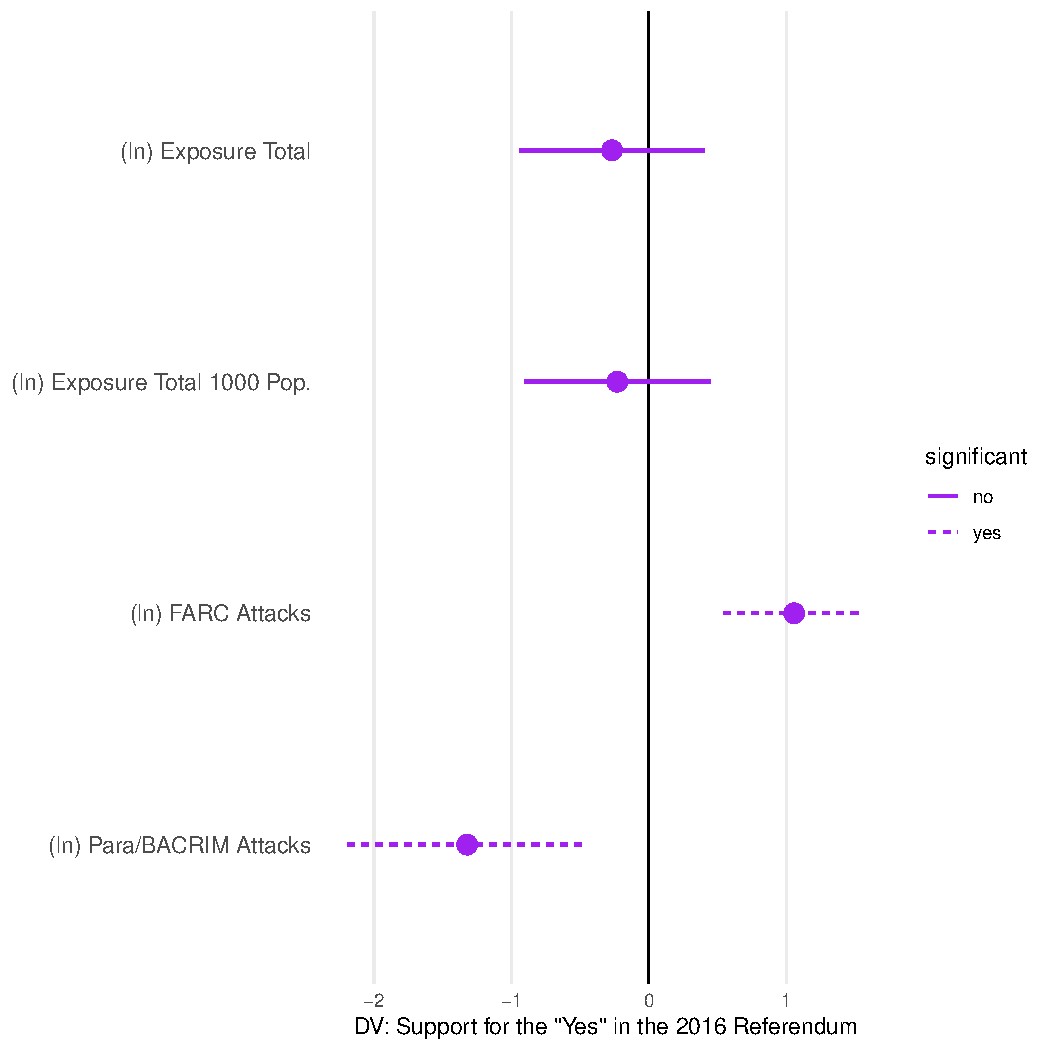
\includegraphics[width=0.8\textwidth, height=12cm]{figure_1.pdf}
	\end{figure}
	
	From this figure \ref{fig:lollipop}, the authors stated that "overall levels of violent attacks by all armed groups in each Colombian municipality do not have an impact on citizens' support for the peace agreement, clear (and statistically significant) effects emerge when we disaggregate by the identity of the perpetrator." These results substantiated their claim that it was important to disaggregate exposure to violence when looking at reasoning behind the 2016 referendum results, as overall exposure to violence was not a significant predictor in support for the referendum.
	
	\clearpage
	
	\section*{4. My Contribution}
	
	\lstinputlisting[language=R, firstline=380, lastline=434]{replication_r_code.R}
	
\end{document}